\chapter{Tutorial 2: computing time calculation}


In that tutorial we will see how to calculate the time computation of a script in \xlp with the use of the trigger parameter and xlpTime function.

\section{A script}

Here the script that we will test:

\

for x in range(0,\_1):

 print x
 
 
\section{Linking functions with the trigger parameter}

In order to compute the time, we need to make a call to xlpTime twice:
\begin{itemize}
\item one before the call to the script
\item one after the execution of the script.
\end{itemize}

\

In order to allow synchronisation we will make the first call to xlpTime will be linked to a cell trigger by the use of the parameter trigger. The execution of the script wil be linked to the result of the first call at xlpTime via the trigger parameter. Finally the last call to xlpTime will be linked to the result of the script.

\

Here the result:

\

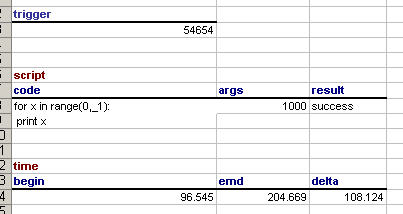
\includegraphics[width=12cm]{images/timecomp.jpg}

\

